% !TEX TS-program = XeLaTeX
% use the following command:
% all document files must be coded in UTF-8
\documentclass[english]{textolivre}
% build HTML with: make4ht -e build.lua -c textolivre.cfg -x -u article "fn-in,svg,pic-align"

\journalname{Texto Livre}
\thevolume{16}
%\thenumber{1} % old template
\theyear{2023}
\receiveddate{\DTMdisplaydate{2023}{3}{26}{-1}} % YYYY MM DD
\accepteddate{\DTMdisplaydate{2023}{6}{26}{-1}}
\publisheddate{\DTMdisplaydate{2023}{8}{7}{-1}}
\corrauthor{Jaciluz Dias Fonseca}
\articledoi{10.1590/1983-3652.2023.45482}
%\articleid{NNNN} % if the article ID is not the last 5 numbers of its DOI, provide it using \articleid{} commmand 
% list of available sesscions in the journal: articles, dossier, reports, essays, reviews, interviews, editorial
\articlesessionname{articles}
\runningauthor{Fonseca et al.} 
%\editorname{Leonardo Araújo} % old template
\sectioneditorname{Daniervelin Pereira}
\layouteditorname{Thaís Coutinho}

\title{The animation ``Purl'': an analysis from the perspective of Sociointeractional Semiotics}
\othertitle{A videoanimação ``Purl'': uma análise na perspectiva da Semiótica Sociointeracional}
% if there is a third language title, add here:
%\othertitle{Artikelvorlage zur Einreichung beim Texto Livre Journal}

\author[1]{Jaciluz Dias Fonseca~\orcid{0000-0002-0699-921X}\thanks{Email: \href{jaciluz.fonseca@ufla.br}{jaciluz.fonseca@ufla.br}}}
\author[2]{Helena Maria Ferreira~\orcid{0000-0002-8749-5426}\thanks{Email: \href{helenaferreira@ufla.br}{helenaferreira@ufla.br}}}
\author[3]{Marta Cristina da Silva~\orcid{0000-0003-1917-1734}\thanks{Email: \href{marta.silva@ufjf.br}{marta.silva@ufjf.br}}}
\author[4]{Isabela Vieira Lima~\orcid{0000-0003-1749-0029}\thanks{Email: \href{isabelavieiralima_@hotmail.com}{isabelavieiralima\_@hotmail.com}}}
\affil[1]{Federal University of Lavras, Pro-Rectory of People Management, Lavras, Minas Gerais, Brazil.}
\affil[2]{Federal University of Lavras, Faculty of Human Sciences, Education and Languages, Department of Language Studies, Lavras, Minas Gerais, Brazil.}
\affil[3]{Federal University of Juiz de Fora, Faculty of Letters, Juiz de Fora, Minas Gerais, Brazil.}
\affil[4]{Federal University of Alfenas, Institute of Human Sciences and Letters, Alfenas, Minas Gerais, Brazil.}


\addbibresource{article.bib}
% use biber instead of bibtex
% $ biber article

% used to create dummy text for the template file
\definecolor{dark-gray}{gray}{0.35} % color used to display dummy texts
\usepackage{lipsum}
\SetLipsumParListSurrounders{\colorlet{oldcolor}{.}\color{dark-gray}}{\color{oldcolor}}

% used here only to provide the XeLaTeX and BibTeX logos
\usepackage{hologo}

% if you use multirows in a table, include the multirow package
\usepackage{multirow}

% provides sidewaysfigure environment
\usepackage{rotating}

% CUSTOM EPIGRAPH - BEGIN 
%%% https://tex.stackexchange.com/questions/193178/specific-epigraph-style
\usepackage{epigraph}
\renewcommand\textflush{flushright}
\makeatletter
\newlength\epitextskip
\pretocmd{\@epitext}{\em}{}{}
\apptocmd{\@epitext}{\em}{}{}
\patchcmd{\epigraph}{\@epitext{#1}\\}{\@epitext{#1}\\[\epitextskip]}{}{}
\makeatother
\setlength\epigraphrule{0pt}
\setlength\epitextskip{0.5ex}
\setlength\epigraphwidth{.7\textwidth}
% CUSTOM EPIGRAPH - END

% LANGUAGE - BEGIN
% ARABIC
% for languages that use special fonts, you must provide the typeface that will be used
% \setotherlanguage{arabic}
% \newfontfamily\arabicfont[Script=Arabic]{Amiri}
% \newfontfamily\arabicfontsf[Script=Arabic]{Amiri}
% \newfontfamily\arabicfonttt[Script=Arabic]{Amiri}
%
% in the article, to add arabic text use: \textlang{arabic}{ ... }
%
% RUSSIAN
% for russian text we also need to define fonts with support for Cyrillic script
% \usepackage{fontspec}
% \setotherlanguage{russian}
% \newfontfamily\cyrillicfont{Times New Roman}
% \newfontfamily\cyrillicfontsf{Times New Roman}[Script=Cyrillic]
% \newfontfamily\cyrillicfonttt{Times New Roman}[Script=Cyrillic]
%
% in the text use \begin{russian} ... \end{russian}
% LANGUAGE - END

% EMOJIS - BEGIN
% to use emoticons in your manuscript
% https://stackoverflow.com/questions/190145/how-to-insert-emoticons-in-latex/57076064
% using font Symbola, which has full support
% the font may be downloaded at:
% https://dn-works.com/ufas/
% add to preamble:
% \newfontfamily\Symbola{Symbola}
% in the text use:
% {\Symbola }
% EMOJIS - END

% LABEL REFERENCE TO DESCRIPTIVE LIST - BEGIN
% reference itens in a descriptive list using their labels instead of numbers
% insert the code below in the preambule:
%\makeatletter
%\let\orgdescriptionlabel\descriptionlabel
%\renewcommand*{\descriptionlabel}[1]{%
%  \let\orglabel\label
%  \let\label\@gobble
%  \phantomsection
%  \edef\@currentlabel{#1\unskip}%
%  \let\label\orglabel
%  \orgdescriptionlabel{#1}%
%}
%\makeatother
%
% in your document, use as illustraded here:
%\begin{description}
%  \item[first\label{itm1}] this is only an example;
%  % ...  add more items
%\end{description}
% LABEL REFERENCE TO DESCRIPTIVE LIST - END


% add line numbers for submission
%\usepackage{lineno}
%\linenumbers

\begin{document}
\maketitle

\begin{polyabstract}
\begin{abstract}
Considering the assumption that the primary responsibility of educational institutions is to develop citizens, we understand that the discussion of sometimes controversial topics can contribute to the refinement of social relations. We argue that the animation genre can be an excellent resource to encourage this type of reflection in a playful and appealing way. Therefore, this text analyzes the short film \textcite{purl}, which addresses the theme of sexism in the corporate world. To this end, we adopt the sociointeractional semiotics analysis model as our theoretical framework, developed by \textcite{leal2011organizaccao}, based on concepts from socio-discursive interactionism - SDI \cite{bronckart2012} and the grammar of visual design - GVD \cite{kress2006reading}. At the end of the article, we present considerations regarding the possibilities of working with multiliteracies, using animation as a tool for working with language practices in the classroom, guided by a perspective that can effectively contribute to the development of critical subjects and citizens. 

\keywords{Animation genre \sep Sociointeractional semiotics analysis model \sep Multiliteracies}
\end{abstract}

\begin{portuguese}
\begin{abstract}
 Considerando a premissa de que a responsabilidade precípua das instituições escolares é a de formar cidadãos, entendemos que a discussão sobre temas como o da animação analisada nesta pesquisa pode contribuir para a qualificação das relações sociais, mesmo sendo assuntos que suscitem polêmicas. Nesse sentido, defendemos que o gênero videoanimação pode ser um excelente recurso para motivar esse tipo de reflexão, de modo lúdico e atraente. Assim, objetivamos, com este texto, propor uma análise do curta \textcite{purl}, que aborda a temática do machismo no mundo corporativo. Para tanto, utilizamos como referencial teórico o modelo de análise da Semiótica Sociointeracional, elaborado por \textcite{leal2011organizaccao}, tendo como referência conceitos do Interacionismo Sociodiscursivo - ISD \cite{bronckart2012} e da Gramática do Design Visual - GDV \cite{kress2006reading}. Ao final do artigo, apresentamos considerações acerca das possibilidades do trabalho com os multiletramentos, utilizando a videoanimação como ferramenta para o trabalho com as práticas de linguagem em sala de aula, pautando-se em uma perspectiva que possa, efetivamente, contribuir para a formação de sujeitos críticos e cidadãos.

\keywords{Gênero videoanimação \sep Modelo de análise Semiótico Sociointeracional \sep Multiletramentos}
\end{abstract}
\end{portuguese}
% if there is another abstract, insert it here using the same scheme
\end{polyabstract}

\section{Introduction}

Social interactions are intrinsically related to the uses of language. As such, learning the social ways of doing also entails learning the social ways of saying \cite{bakhtin2011estetica}. It is thus important to problematize generalized and naturalized discourses in order to refine teaching and learning processes and actions in society. According to \textcite{kress2006reading}, when subjects produce or interpret discourses, they make choices that are directly related to their social experiences, which inevitably transform them into reproducers of certain prototypical models that circulate socially.

In the labor context, for example, situations involving discrimination related to ethnicity, race, gender, age, nationality, sexual orientation, social status, religion, or even disability are quite prevalent. There is a commonplace practice of emphasizing values of pre-established standards rather than the ability to perform social roles.

In this context, the computer-animated film Purl was created to provoke reflections about discrimination against women. With this study, we seek to analyze which verbal and nonverbal resources are used to create the effects of meaning pursued by such an animation. Released in 2018 on YouTube, directed by Kristen Lester and produced in a partnership between Disney and Pixar, the short film begins with a pink ball of yarn arriving at an investment office where the employees are exclusively men wearing black suits. The environment is characterized by the reinforcement of a prototypical model culturally associated with the male universe, such as aggressiveness. Purl, a name that makes reference to a knitting stitch, attempts to become part of this environment by any means necessary, and when she succeeds, she finds herself in a dilemma with the arrival of a new employee: a yellow ball of yarn named Lacy.

For the analysis proposed here, we adopted the sociointeractional semiotics analysis model developed by \textcite{leal2011organizaccao} as our theoretical framework, which can offer a deeper understanding of multimodal genres. \textcite{purl} was selected given the importance of the animation genre in language classes, usually suitable for approaching a range of different topics, such as sexism in the labor market.


\section{Sociointeractional semiotics analysis model}

The framework we selected to support the analysis of \textcite{purl} was developed by \textcite{leal2011organizaccao}, based on the tenets of socio-discursive interactionism (SDI), as proposed by \textcite{bronckart2012}, and the conceptions of the grammar of visual design (GVD), a theory developed by \textcite{kress2006reading}. 

 The two theories favored the establishment of a methodological model that analyzes the role of different sign systems in the performance of human activities, as well as the textual production/reception in a context analysis, namely, the sociointeractional semiotics analysis model. This model is divided into three parts: textual reception; nonverbal language and its interaction with verbal language; and a reconstruction of the SDI analysis model, to which \textcite{leal2011organizaccao} added the categories proposed by the GVD. In \Cref{tab1}, we present an overview of the sociointeractional semiotics analysis model.


\begin{table}[h!]
\caption{Overview of the sociointeractional semiotics analysis model.}
\label{tab1}
\begin{tabular}{cccp{3cm}p{3cm}p{5.5cm}}
\toprule
 \parbox[t]{2mm}{\multirow{10}{*}{\raisebox{-3.5\height}{\rotatebox[origin=c]{90}{RELATED ACTIVITY/ACTIVITIES}}}} & 
 \parbox[t]{2mm}{\multirow{10}{*}{\raisebox{-3\height}{\rotatebox[origin=c]{90}{GENRE SELECTED MEDIUM DEFINED}}}} & 
 %\parbox[t]{2mm}{\multirow{4}{*}{\rotatebox[origin=c]{90}{Language action}}} 
 \multirow{4}{*}{\raisebox{-3.5\height}{\rotatebox[origin=c]{90}{Language action}}}
 & \multirow{2}{*}{Production context} & Physical context & 
 \begin{itemize}
     \item Place of production 
     \item Moment of production
     \item Producer
     \item Receiver
 \end{itemize}
 \\ \cline{5-6} 
 &  &  &  & Socio-subjective context & 
 \begin{itemize}
     \item Social place of production
     \item Social position of producer and receiver
     \item Objective
 \end{itemize}
  \\ \cline{4-6} 
 &  &  & \multirow{2}{*}{Reception context} & Physical context & 
 \begin{itemize}
     \item Place of reception
     \item Moment 	of reception
     \item Receiver
     \item Producer
 \end{itemize} \\ \cline{5-6} 
 &  &  &  & Socio-subjective context & 
 \begin{itemize}
     \item Social place of reception
     \item Social position of receiver and producer
     \item Objective
 \end{itemize} \\ \cline{3-6} 
 &  & \parbox[t]{2mm}{\multirow{6}{*}{\raisebox{-2\height}{\rotatebox[origin=c]{90}{Internal Architecture of the Texts}}}} & \multirow{2}{=}{Thematic-representational 			organization} & Verbal thematic representational organization & \begin{itemize}
     \item Types of discourse
 \end{itemize} \\ \cline{5-6} 
 &  &  &  & Nonverbal thematic representational organization & \begin{itemize}
     \item Types of representation
 \end{itemize} \\ \cline{4-6} 
 &  &  & \multirow{2}{=}{Interactional organization} & Verbal expression & Discourse voices Modality \\ \cline{5-6} 
 &  &  &  & Nonverbal expression & \begin{itemize}
     \item Contact
     \item Social distance
     \item Attitude
     \item Modalization
 \end{itemize}  \\ \cline{4-6} 
 &  &  & \multirow{2}{=}{Structural organization} & Verbal organization & \begin{itemize}
     \item Connection
     \item Nominal cohesion
 \end{itemize} \\ \cline{5-6} 
 &  &  &  & Nonverbal organization & 
 \begin{itemize}
     \item Information value
     \item Salience
     \item Framing
 \end{itemize} \\ 
\bottomrule
\end{tabular}
\source{\textcite[p. 212]{leal2011organizaccao}}
\end{table}

With regard to textual reception, \textcite{leal2011organizaccao} begins with the notion that texts, as a process of interaction, have two sides: textual production and reception, i.e., the processes of reading and understanding or interpretation, and the context of the text reception. Three elements are essential for the language action to take place, including the producer, the text, and the reader, with the interaction among them underpinning the  language processes. For SDI, the language action is determined by four factors: I. the production context, the situation that the agent producing the text believes to exist (but whose real production situation cannot be truly accessed, although it can be inferred from clues available in the text); II. the thematic content,  the set of information explicitly presented in the text; III. the recognition of the genre; and IV. the identification of the language activity, with the latter two deriving from the formal and functional characteristics of the text.

Drawing on SDI, \textcite{leal2011organizaccao} performs context analysis along two pathways: the production context and the reception context. The production context, based on concepts from SDI, encompasses, as shown in \Cref{tab1}, the physical context, which involves the place and moment of production, as well as the producer and receiver of the text and the socio-subjective context, including the social place of the production, the social position of the producer and receiver, and the objective. \textcite{leal2011organizaccao} also adds to this analysis the activity in which the text was produced, the genre selected for the production, and the medium defined for publication. 

Producing a text goes beyond the activity of communicating and expressing thoughts, for it involves taking a position on what was uttered. Producing a text means saying something to someone, for some reason, in some way, in a given interaction situation. When producing a text, the subjects take a dialogical position toward the interlocutors. In turn, the reception context is based on the interpreter’s viewpoint, who has a purpose for reading. It also includes activity, textual genre, physical context (with the place and moment of reception, producer and receiver), and socio-subjective context (with the social place of the receiver, the social position of the receiver and producer, and the objective). Thus, through the clues constitutive of the producers’ project of saying, the reader makes associations, for which they mobilize prior knowledge. 

The context is organized by the linguistic dimension and the situational dimension (socio-historical-cultural situation) in an inextricable way, for the process of the subjects’ integration into the social group takes place in and through language. 

The perception of the thematic content is thus the product of inferences drawn from that prior knowledge. In other words, the thematic content is the knowledge of the individual that was acquired in the social and cultural environment expressed in the text, which is retrieved by the receiver at the moment of reading. As such, the relationship between context and prior knowledge makes it possible to understand the text and assimilate inferences, as well as to retrieve — in the textual reception — the configurations of the representations constructed by the author of the text. 

Assuming that texts are multimodal artifacts, \textcite{leal2011organizaccao} links the conceptions\footnote{Given space limitations, for further information on the subject and a more detailed explanation of the concepts used in SDI and the GVD, please see \textcite{bronckart2012} and \textcite{kress2006reading}, respectively.} of textual architecture in SDI \cite{bronckart2012} to those of metafunctions in the GVD \cite{kress2006reading}, resulting in what she calls \textbf{sociointeractional semiotics}, in which the linguistic dimension interacts with the other semiotics. The thematic and discursive organizations of the infrastructure layer in SDI are related to the narrative and conceptual processes of the representational metafunction of the GVD, producing thematic-representational organization, which addresses the ways of placing social representations in discourse that can be either verbal or nonverbal. 

Verbal thematic-representational organization is focused on “how the thematic content of the text is organized in its linguistic externalizations” \cite[p. 206]{leal2011organizaccao}, through the types of discourse proposed by \textcite{bronckart2012}, namely, interactive discourse and theoretical discourse (at the expository level), and interactive report and narration (at the narrative level). In turn, nonverbal thematic-representational organization encompasses the types of representation developed by \textcite{kress2006reading}, which can be narrative or conceptual. To analyze the animation \textcite{purl}, we focus on interactive discourse and narration, as well as conceptual representations\footnote{The sociointeractional semiotics analysis model was developed by \textcite{leal2011organizaccao} to analyze the cartoon genre, which is distinct from the animation genre, particularly because the basic characteristics of the latter include movement and scenic sequences. Nonetheless, we found points of convergence, as both express meanings through the relationship between images and words (or solely images). We thus consider it appropriate to use Leal’s (2011) model to analyze animation.}. 

According to \textcite{leal2011organizaccao}, with regard to enunciative responsibility, the distribution of voices and modality which comprise the layer of enunciative mechanisms in SDI, are intrinsically linkeded. These elements are related to contact, social distance, perspective and modality in the interactive metafunction of the GVD, resulting in interactional organization, i.e., the ways of expressing the interaction, which may be verbal or nonverbal.

Verbal interactional organization is expressed through discourse voices and modalization, while nonverbal interactional organization involves contact (exposition or interpellation); social distance, through film shots (close-up, medium, or wide); attitude (subjective or objective); and modality, with the use of color, contextualization, and caricatured representation. In our analysis, we focus on modalization and modality.

Finally, the layer that deals with the mechanisms of textualization in SDI, which includes the relationships of connection and nominal cohesion, is linked to the compositional metafunction of the GVD, which includes information value, salience and framing. In sociointeractional semiotics \cite{leal2011organizaccao}, this results in structural organization, which can also be verbal or nonverbal.

Verbal structural organization thus includes elements of connection and nominal cohesion, while nonverbal structural organization is presented through information value, which can be centered or isolated in the scene; salience (minimum or maximum); and framing, as the frame can connect or disconnect scenic elements, depending on its use. In \textcite{purl}, our gaze turned to elements of connection and information value. We will now proceed to the analysis of the animation, guided by the framework presented. 


\section{\emph{Purl} and sexism in the corporate world}

Considering the sociointeractional semiotics analysis model, we selected several scenes\footnote{The images used in this article are exclusively for educational, non-profit purposes, falling under the policy of fair use of media for the development of citizens \cite{brasil2009, youtube}.} from \textcite{purl} to demonstrate how this approach can contribute to understanding the effects of meanings that can be elicited from the audience of the animation genre. We demonstrate below how the aspects indicated by the author can be applied to the Disney-Pixar short film. 

With regard to the production context, \textcite{purl} was produced in partnership between media company Disney and digital animation company Pixar. This was their first production distributed directly online. The short film was directed by Kristen Lester and made part of the SparkShorts project, which seeks to discover new filmmaking talent \cite{penzani2019}. 

Lester explains that the idea for \textcite{purl} came from her own experience as one of the few female animators in a predominantly male environment \cite{meet2019}. The animation was thus created to stimulate reflection about toxic masculinity in the workplace. The short film is set in an office, and the narrative deals with the relationship between the employees who had already been working there and the new female employee, who attempts to be accepted in that environment. 

As Disney and Pixar are internationally acclaimed companies, the production is embedded in a context that should be problematized. In addition to the technical conditions (high-tech resources, skilled professionals, a tradition of film production, etc.), both production companies are leaders in addressing social issues and engaging with movements related to diversity. 

According to \textcite{wells1998}, animation has a narrative organization that exhibits a light, casual tone, even when it proposes to make a social critique by using satire and humor. This characteristic is essential to mobilizing the audience’s interest in issues that can be difficult to grasp and addressing questions related to social responsibility. Considering the perspective that to produce a text is to act, in the context of a given social activity, animation is a way to construct a point of view, to give meaning to a project of saying, in its relationship with the recipient(s), objective, space and moment of production, and the organizational characteristics (plane of the text, mechanisms of textualization, and enunciative mechanisms) associated with the textual genre in question. 

The reception context is based on a conception of language as a situated practice. The reception, according to \textcite{leal2011organizaccao}, includes not only the processes of understanding/interpretation but also the subject-reader, who — in the same way as the producer — is crucial to the process of meaning production. The receiver also acts in that process based on his/her social experiences. For the author, those who interpret a text do so based on their universe of knowledge, including making it more current. 

In this context, the animation under analysis demonstrates a tendency that is recurrent in studies on the genre: to encompass different interlocutors simultaneously. For \textcite[p.~75]{gomes2007double}, “[...] contemporary cartoons have woven a denser and more multifaceted narrative structure, marked by intertextual references, parodies, satires, and a new social landscape that situates the child and the adult within the same work [...]”. 

With the democratization of internet access and the globalization of interactions via social networks, animation has begun to circulate more broadly, reaching different audiences. Consequently, when developing educational practices, it is necessary to consider the age group, the course objective, and the nature of the interactions. It is important to think about the fact that the didactic work proposed by the teacher will influence how students will interact with the texts. The discussion may address different themes: gender inequality, sexism, toxic masculinity, labor relations, etc. We suggest working with students in middle and high school, in language classes, although interdisciplinary work is also recommended. 

As \textcite{leal2011organizaccao} states, the thematic-representational organization of the text is based on the relationship between its verbal and nonverbal aspects\footnote{The groups proposed by \textcite{leal2011organizaccao} for the representational, interactional, and structural organization of the verbal and non-verbal aspects are merely one way to facilitate the analysis of multimodal texts, as those elements are imbricated in and permeate one another at all times, in order to establish the effects of meaning sought by the text.}. In \textcite{purl}, narration and interactive discourse are the predominant types of discourse. Narration arises from the organization into a narrative sequence, considering that it is a linearly structured story, beginning with an initial situation (Purl arrives at the office), followed by a complication (Purl is not accepted by her colleagues) and actions that lead to a resolution (she changes her look and her attitudes), until arriving at a final situation (she is accepted, embraces a new colleague, and changes the paradigm of the entire office).

Interactive discourse appears throughout the animation, as the story unfolds through dialogs between the characters. However, the meaning intended by the animation does not result only from the types of discourse used, but rather from the relationship they establish with the images that make up the animation scenic sequences. Although there is no narrator telling the story, it is possible to infer the meanings proposed by the story through the images and the relationship between them and the characters’ lines. An example of this relationship can be seen in the opening and closing scenes.

The animation opens in a spatial setting: the camera shows an office full of white men wearing suits in small groups: two make plans to go to the gym together, three are by the water fountain laughing at what appears to be a joke, and half a dozen are arguing in a conference room. Then, there is a wide shot showing the entire office, and a man’s voice can be heard welcoming a new employee, as yet unseen. 

The man says: “You’ll be up on the fourth floor with investments....” However, his introduction is interrupted when he reads something on his cell phone, saying: “What? The Tigers are up by 20? Yes!” and makes a gesture of victory. He then continues: “Anyway, it’s entry level, but your resume was by far the strongest,” and picks up the badge to hand to the new employee. When he sees the photo, he makes a startled expression and looks down, at which point the camera reveals that the new employee is a pink ball of yarn: Purl. 

She seems excited, saying that being there is “Unbelievable,” to which the man replies: “Unbeweavable.” Here, it is possible to see the use of inference, as the young man makes a pun with the word “weave,” as if the scene could not be weaved, i.e., created, could not be real. As \textcite[p. 165]{leal2011organizaccao} reminds us of, “the production of inferences has an essential role in the recognition and construction of meanings, for the reader’s knowledge is central to the creation of different understandings for a single text.” It is an allusion to Purl being a ball of yarn, which can only be understood if the reader infers the meaning of the scene based on the relationship between word and image. Next, the elevator door opens, and Purl walks into the office and is stared at in surprise by the men, as in \Cref{fig1}.

\begin{figure}[htbp]
\centering
\begin{minipage}{.7\textwidth}
 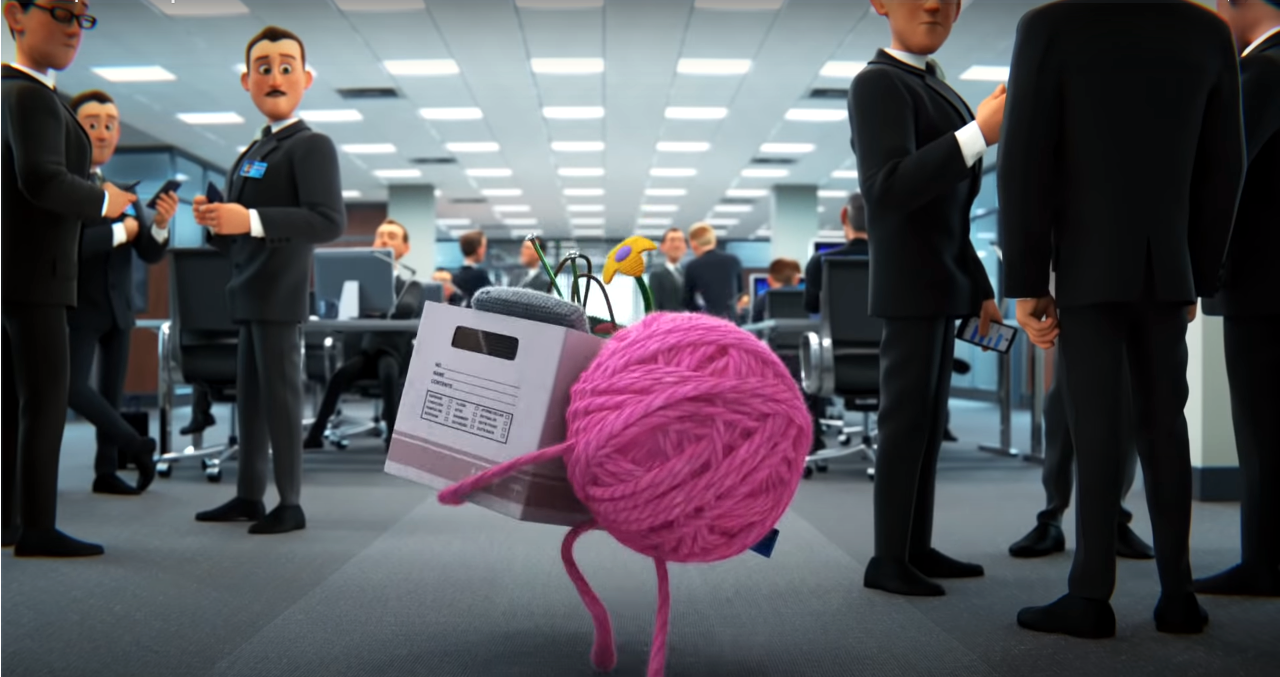
\includegraphics[width=\textwidth]{Fig1.png}
 \caption{Opening scene shows how images and words contribute to the understanding of the animation’s thematic-representational organization.}
 \label{fig1}
 \source{frame at 1:22 of \textcite{purl}.}
\end{minipage}
\end{figure}

We understand that the young man’s reference to the Tigers (an American baseball team) can be seen as a way for the animation to associate the male universe with sports, seeking to show elements that are culturally associated with men. In addition, that meaning is complemented by the images of all the men wearing black suits, divided into small groups, making plans to work out, laughing at jokes and being aggressive, such that all those elements contribute to characterizing the environment as male. It is placed in opposition to the pink ball of yarn, carrying a box with elements that are culturally associated with the female universe (lilac mug, yarn, and knitting needles), which is complemented by the surprised expressions of the men in the office. 

Those expressions help convey the types of representation used in animation, which, as \textcite{leal2011organizaccao} explains, can be narrative or conceptual. Narrative representations are largely expressed through actions and gazes, and their analysis thus requires a greater level of detail, which is hindered by the necessary brevity of this text. We thus turn our focus to conceptual representations and, more specifically, to the symbolism present in the animation through the colors used. 

In the short film, pink is used to symbolize the female, in opposition to the gravitas imposed by the color black, which symbolizes the male. We understand that this cliché is portrayed precisely to provoke an interrogation about how society associates colors with genders, to such an extent that in order for Purl to become part of the group, she has to disassociate herself from the pink ball of yarn, transforming herself into a rectangular being wearing a black suit that she knits for herself, similar to the ones worn by the men in the office. 

This allows us to proceed to the analysis of the animation’s interactional organization. To illustrate that use, we have chosen two moments in which the staff meet to talk about the company’s performance. The scene opens with the leader of the meeting presenting a pie chart (\Cref{fig2}) and saying: “As you can see, we’ve got a big, fat...,” at which point the camera moves away and the word “FAILURE” appears, in red, as the man says: “...failure.” The pause after the word “fat” builds up anticipation and takes on an ironic meaning, when it is associated with the title of the presentation. This is an example of the use of modalization in verbal language. 

\begin{figure}[htbp]
\centering
\begin{minipage}{.7\textwidth}
 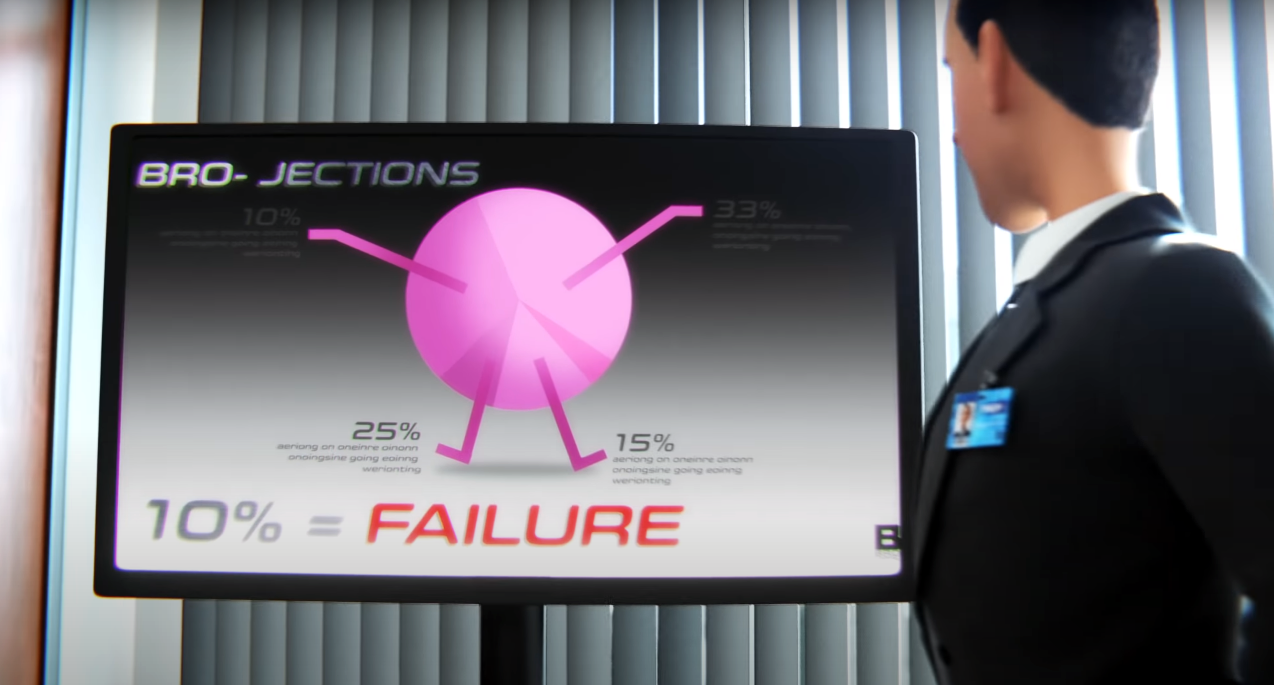
\includegraphics[width=\textwidth]{Fig2.png}
 \caption{The first presentation of the company’s projections contributes to understanding the animation’s interactional organization.}
 \label{fig2}
 \source{frame at 2:51 of \textcite{purl}.}
\end{minipage}
\end{figure}

Furthermore, in terms of the other semiotics, the shape and color of the pie chart are reminiscent of Purl, evoking the idea that her arrival is a failure. This meaning is reinforced through a comparison with a later scene, in which the same effect is used but now with a positive meaning. After Purl begins wearing a suit similar to her colleagues’ and starts to become part of the group, there is another staff meeting. 

It opens with the presentation of a new graph, this time an area chart (\Cref{fig3}), with the leader in the background saying, “These results speak for themselves,” as the camera pans away from the graph, showing the word “SUCCESS!” in yellow. The area chart now resembles the shape of Purl wearing a suit, which makes it possible to associate this new look with her success in the company, after she has changed in pursuit of acceptance.

\begin{figure}[htbp]
\centering
\begin{minipage}{.7\textwidth}
 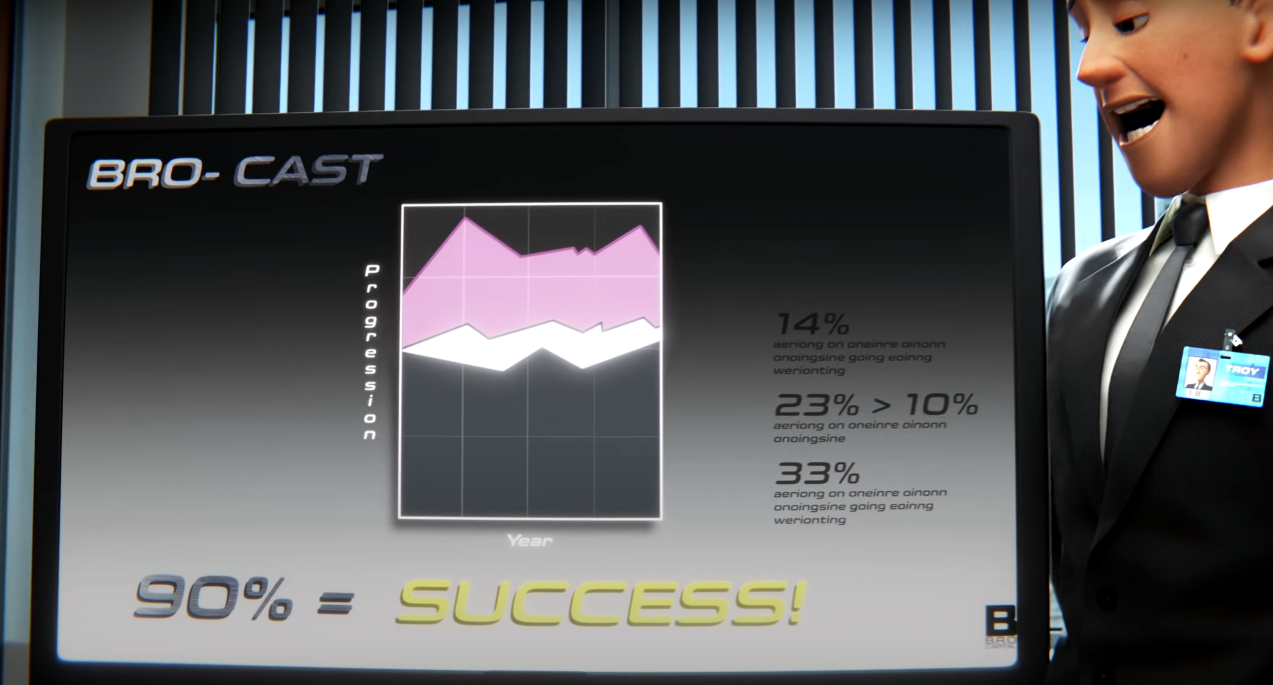
\includegraphics[width=\textwidth]{Fig3.png}
 \caption{The second presentation of the company’s projections reinforces the understanding of the animation’s interactional organization.}
 \label{fig3}
 \source{frame at 5:02 of \textcite{purl}.}
\end{minipage}
\end{figure}

The pie and area charts, associated with the words “failure” and “success,” are an example of the use of modality, as the meanings can be deduced through the colors, and a contextualization related to the characterization of Purl, functioning as a caricatured representation of her. Firstly a round, pink chart is used, similar to the spherical shape and color of Purl at the beginning of the narrative, accompanied by the word “failure” in red, a color culturally associated with risk and financial loss (“being in the red” is synonymous with lacking money). In addition, at a second moment, there is a pink, white and black chart, similar to Purl dressed in a suit, accompanied by the word “success” in yellow, a color traditionally associated with money and wealth. 

The relationship between these two scenes can also be seen as an example of the animation’s structural organization, given that the images function as an element of connection, through the reiteration and reinforcement of an idea. However, along these lines, we indicate another example. The narrative unfolds using a repetition of the situations experienced by Purl, in order to demonstrate that when she was dressed as a ball of yarn and acting in a more delicate way (typically female), she was treated with indifference and exclusion. However, when she was dressed similarly to her colleagues, wearing a suit and tie, and acting aggressively (typically male), she began to be included.

Two elements of connection between those situations can be found in the lines of the team leader. First, after calling the meeting and presenting the data, he says, “Finance wants answers. Ideas?” When Purl suggests teamwork (and even uses the term “knit,” maintaining the relationship with the universe of knitting), she is ignored and pushed into the corner, as in \Cref{fig4}. After the meeting, he invites his colleagues to go out for a drink, leaving Purl behind. When asked if everyone is there, he looks at Purl indifferently, saying, “Yeah, that's everybody,” and they get on the elevator to leave without her. Purl’s sadness at her exclusion is expressed in a scene in which she is depicted as tiny, in a large, empty office (\Cref{fig5}). 

\begin{figure}[htbp]
\centering
\begin{minipage}{.7\textwidth}
 
\includegraphics[width=\textwidth]{Fig4.png}
 \caption{Purl at the margins of the scene illustrates the animation’s structural organization.}
 \label{fig4}
 \source{frame at 3:19 of \textcite{purl}.}
\end{minipage}
\end{figure}

\begin{figure}[htbp]
\centering
\begin{minipage}{.7\textwidth}
 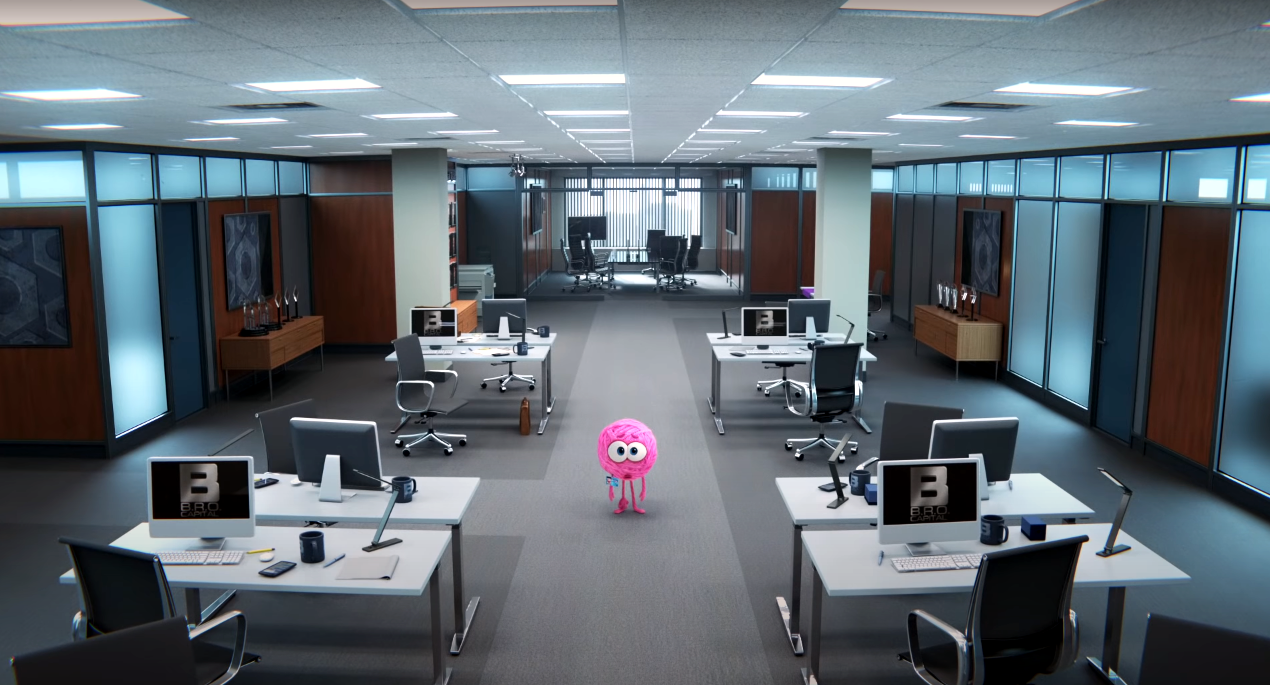
\includegraphics[width=\textwidth]{Fig5.png}
 \caption{A tiny Purl confronted by the vastness of the empty office illustrates the animation’s structural organization.}
 \label{fig5}
 \source{frame at 3:47 of \textcite{purl}.}
\end{minipage}
\end{figure}

The two situations are repeated, but now with Purl wearing a suit. At the next team meeting, following the data presentation, when the boss starts to say “But Finance is still asking for...,” he is interrupted by Purl, who climbs on the table, saying aggressively: “I say we go for it! And if Finance doesn’t like it, they can kiss our ass!”, at which point she is cheered by her colleagues, as shown in \Cref{fig6}. Then, the boss once again invites everyone to go for a drink. As they are leaving, he is asked if everyone is there, and he says: “Hold up. Not everybody.” They walk out surrounding Purl and talking to her, who now feels like one of them, as shown in \Cref{fig7}.

\begin{figure}[htbp]
\centering
\begin{minipage}{.7\textwidth}
 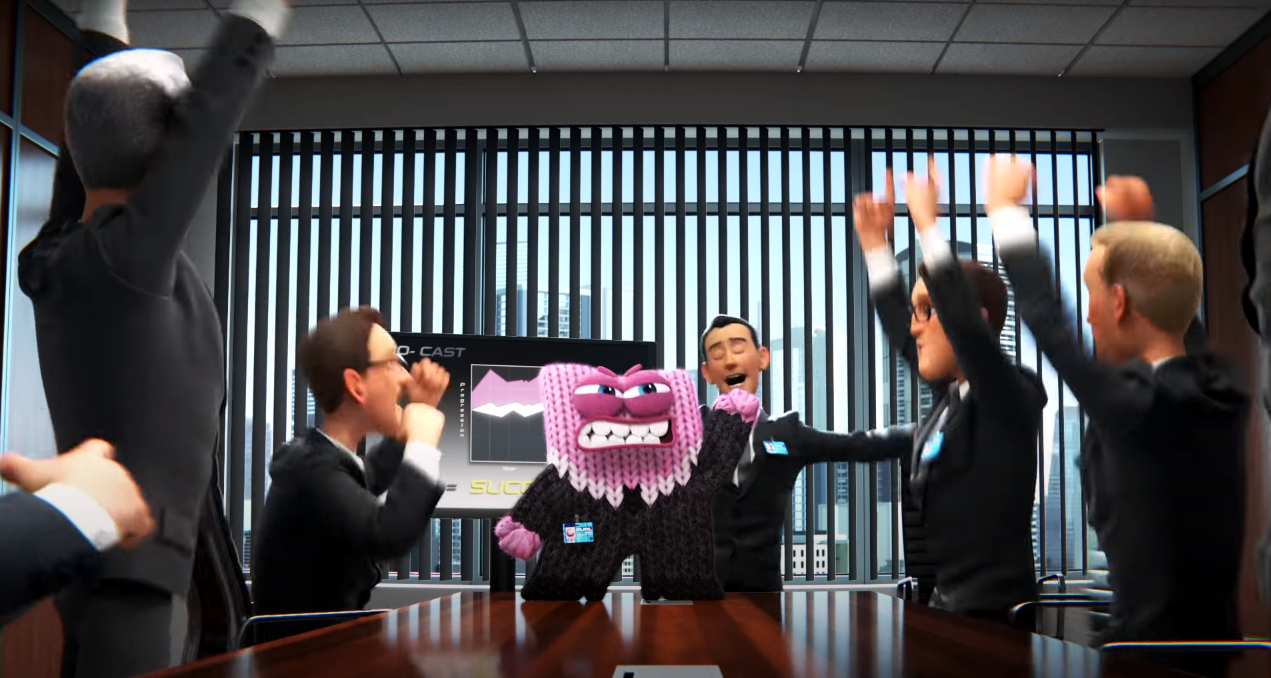
\includegraphics[width=\textwidth]{Fig6.png}
 \caption{Purl in the center of the scene illustrates the animation’s structural organization.}
 \label{fig6}
 \source{frame at 5:11 of Purl \textcite{purl}.}
\end{minipage}
\end{figure}


\begin{figure}[htbp]
\centering
\begin{minipage}{.7\textwidth}
 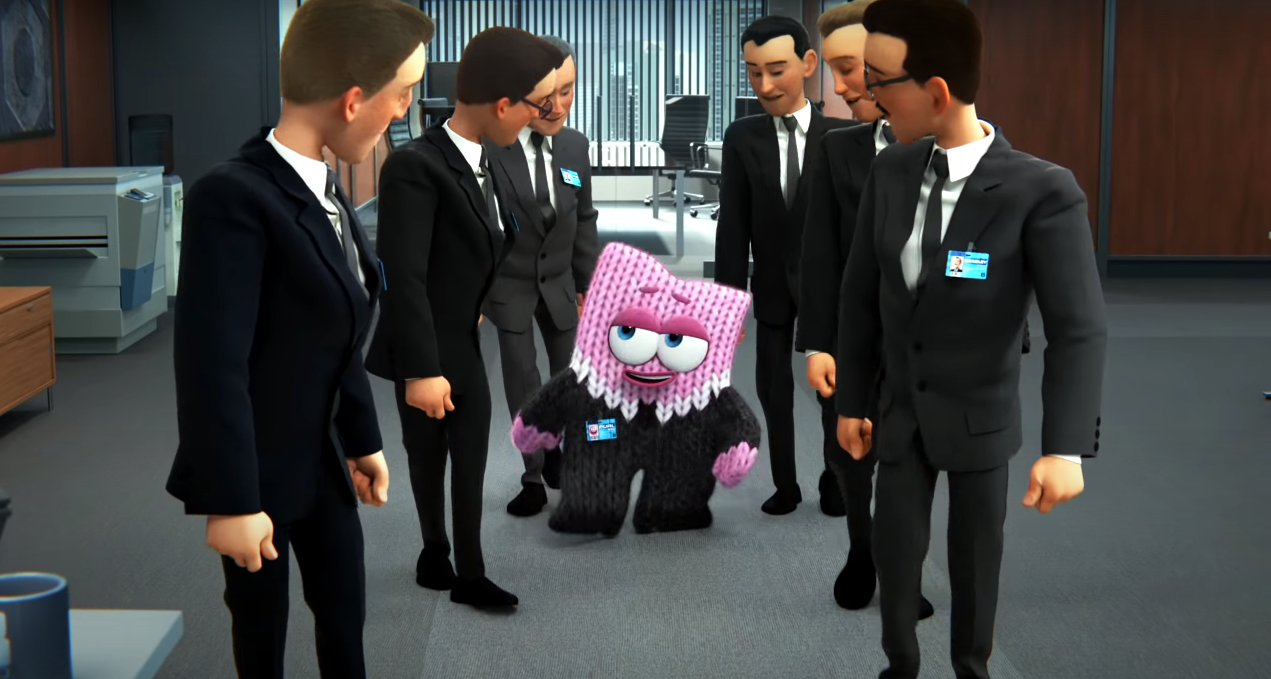
\includegraphics[width=\textwidth]{Fig7.png}
 \caption{Purl flanked by her colleagues illustrates the animation’s structural organization.}
 \label{fig7}
 \source{frame at 5:34 of \textcite{purl}.}
\end{minipage}
\end{figure}

The change in the way Purl’s colleagues treat her is demonstrated by the use of information value in the scenes presented. Although she is sidelined at the beginning, which is expressed by the depiction of her at the margins of the scene (\Cref{fig4}, after she exhibits an aggressive attitude, she is depicted in the middle of the scene (\Cref{fig6}). Along the same lines, the depiction of her sadness and exclusion utilizes a frame in which she is shown as tiny in comparison to the vastness of the office (\Cref{fig5}), while her inclusion is depicted with her in the center of the scene, in a more equal position with her colleagues (\Cref{fig7}). 

However, what is most significant, in our opinion, takes place at the end of the animation. After becoming part of the group of men by acting like them, Purl’s attitude is challenged by the arrival of a new co-worker: Lacy, a yellow ball of yarn. At first, Purl chooses to exclude her, preferring the acceptance of the men. She then looks at her name tag, remembers what she herself experienced, and recognizes herself as equal to her female colleague. She then adopts a new attitude and includes Lacy from the beginning, inviting her to go out with her and her male colleagues.

The scenes that follow evoke the beginning of the narrative, except that now, alongside the men — who no longer wear only black suits — there are several colorful balls of yarn. Now it is Purl who welcomes a new colleague, showing the same excitement as she did when she arrived, expressed by the same lines as at the beginning, only now is it the man who says, “It’s still kind of unbelievable that I’m here,” to which she responds, “I would say it’s unbeweavable.” He, however, is welcomed into a new environment (\Cref{fig8}), now with men and balls of yarn laughing together at the water fountain and chatting amiably in the conference room.

\begin{figure}[htbp]
\centering
\begin{minipage}{.7\textwidth}
 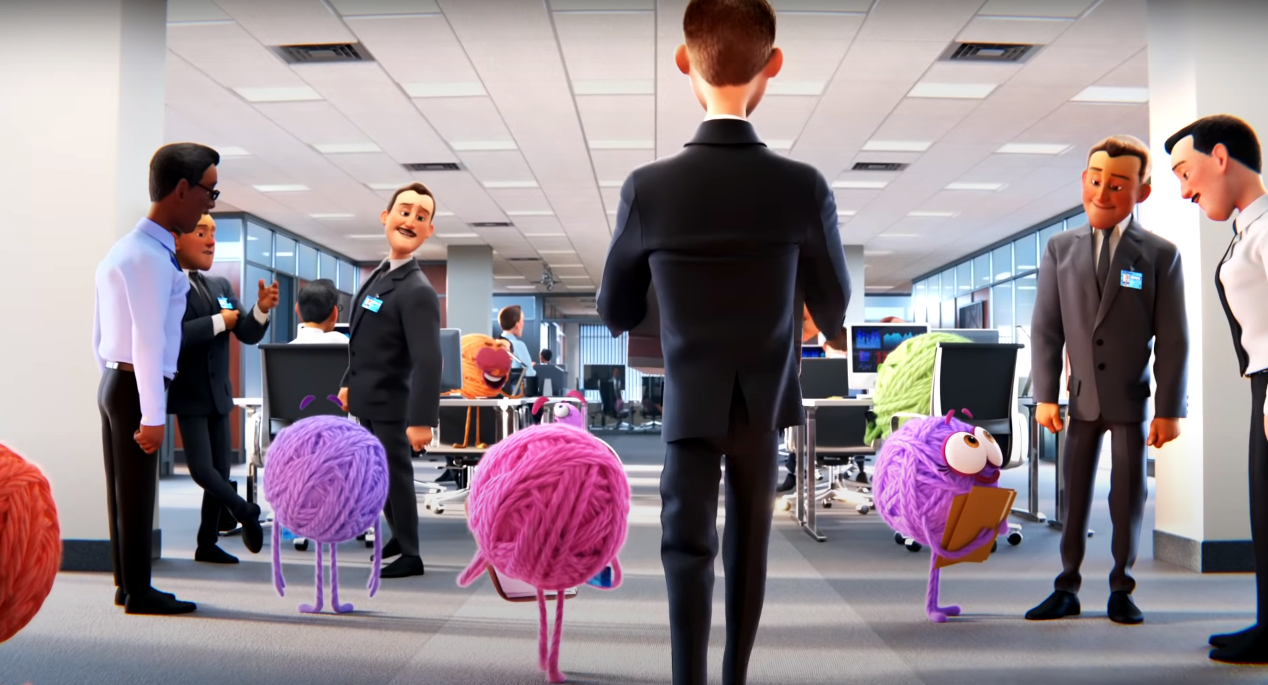
\includegraphics[width=\textwidth]{Fig8.png}
 \caption{Final scene shows Purl’s subversion of order.}
 \label{fig8}
 \source{frame at 7:46 of \textcite{purl}.}
\end{minipage}
\end{figure}

The choice to represent the woman as a ball of yarn can be seen as a symbol for the different one, that which is alien and out of the ordinary, arriving at a place where attitudes and behavior are always the same. The ball of yarn can represent not only women, but black people, Asians, those who are transgender, or anyone outside of a socially imposed norm. In addition, the ball of yarn also alludes to textiles, creating with one’s own hands by knitting, which was mentioned several times throughout the animation. For example, Purl tells a joke at the beginning, which was not well-received by her colleagues, and, in the final line, “Tell us all about yourself. We do love a good yarn, ”the word “yarn” is a colloquialism for talking and chatting, figuratively speaking. 

By subverting the order imposed upon her, Purl is a character who breaks with the logic of sexism that had been prevalent in the office. In addition, the circular narrative, which repeats the same situations, but with the characters expressing different attitudes, contributes to producing the effects of meaning intended by the animation. The analysis of the verbal language associated with the other semiotics (visual and sound) in \textcite{purl} made it possible to understand how the elements that make up the short film were not selected at random but, rather, with a purpose: to present situations that take place in the social context and, with a touch of humor, to provoke a reflection about what we experience in our society. That reflection, guided by an analysis of the different languages, can foster a critical position toward the meanings produced through the reading of the animation. 



\section{Final considerations}

Based on the sociointeractional semiotics analysis model \cite{leal2011organizaccao}, we tried to demonstrate that the proposed analysis can contribute to a better understanding of the effects of meaning created in the short film \textcite{purl}. This makes it possible to engage in discussions about different approaches to language teaching and learning. We understand that the animation genre can be used in the teaching process to encourage students to cast a critical eye on the social context, characterized by an increasingly frequent use of digital technologies.

Problematizing the texts that circulate in the information society, using a perspective that brings together different issues — production context, reception context, thematic - representational organization, interactional organization, and structural organization — can enable an analysis in a theoretically grounded dimension. 

When analyzing the dimension of multimodal text analysis, based on the theoretical assumptions of sociointeractional semiotics, it is necessary to consider basic aspects, such as recognition of the genre, medium, activity in which the text is embedded and the physical and social context. In addition to those issues, the theorization also points to the construction of relationships between the elements of the text, construction of inferences and value judgments (critical position toward the text), perception of the text aims/objectives and its processes and strategies to achieve those objectives. This approach helps identify the types of representation of the different semiotic units related to the thematic content, identify the ways of establishing the types of interaction between the producer and the reader based on the text, and analyze the compositional structure inherent to the text overall organization.

By addressing the characteristics of sexism in the labor market, \textcite{purl} contributes to promoting spaces for discussion that can be instrumental in the formation of critical subjects and helps to mitigate attitudes of discrimination and prejudice that still persist in labor contexts. The development of reading practices that engage the reader, in an approach that links linguistic and semiotic issues, can foster forms of acting critically in society. 

Based on the study conducted, it was possible to consider that the link between SDI and the GVD, proposed by sociointeractional semiotics, points toward possibilities for re-signifying teaching practices for reading in the classroom. By involving the multimodality constitutive of texts, \textcite{leal2011organizaccao} indicates the construction of a nonlinear path for the reading process, in which linguistic aspects and other semiotics are addressed. 

In this interaction, the theoretical construct can — through didactic transposition — encourage the development of activities that enable the refinement of interpretation skills. A pedagogical proposal grounded in the language/action perspective must therefore consider the properties of the formal worlds that exert an influence on the production of a text (production conditions, production context, situationality, project of saying, characteristics of the interlocutors, etc.). Furthermore, it is also possible to consider the analytical categories related to the different dimensions that constitute the process of meaning production (thematic-representational organization, interactional organization, and structural organization). Proposing a didactic approach that considers the processes of the organization and functioning of texts cultivates a more appropriate approach to reading practices in the classroom. 

We thus believe that reading animation is an important strategy for the development of critical readers, as it encompasses different aspects of the textual constitution and the interactions that circulate in digital contexts, demonstrating that texts are configured as discursive projects, laden with meanings. Animation, specifically, is structured to provoke the subject-viewer, negotiating with the constitutive voices of the text and the processes of interaction, in a position of agreement, disagreement, reinforcement and interrogation, and, as a result, constructing their point of view and constituting them as a subject in and through language.



\printbibliography\label{sec-bib}
% if the text is not in Portuguese, it might be necessary to use the code below instead to print the correct ABNT abbreviations [s.n.], [s.l.]
%\begin{portuguese}
%\printbibliography[title={Bibliography}]
%\end{portuguese}


%full list: conceptualization,datacuration,formalanalysis,funding,investigation,methodology,projadm,resources,software,supervision,validation,visualization,writing,review
\begin{contributors}[sec-contributors]
\authorcontribution{Jaciluz Dias Fonseca}[conceptualization,datacuration,investigation,writing,review]
\authorcontribution{Helena Maria Ferreira}[conceptualization,funding,projaadm,writing,review]
\authorcontribution{Marta Cristina da Silva}[formalanalysis,methodology,supervision,writing]
\authorcontribution{Isabela Vieira Lima}[datacuration,investigation,visualization,writing]
\end{contributors}




\end{document}

